\documentclass{article}
\usepackage{listings}
\usepackage{mathrsfs}
\usepackage[utf8]{inputenc}
\usepackage{amssymb}
\usepackage{lipsum}
\usepackage{amsmath}
\usepackage{fancyhdr}
\usepackage{geometry}
\usepackage{scrextend}
\usepackage[english,german]{babel}
\usepackage{titling}
\setlength{\droptitle}{-3cm}
\usepackage{tikz}
\usepackage{algorithm,algpseudocode}
\usepackage[doublespacing]{setspace}
\usetikzlibrary{datavisualization}
\usetikzlibrary{datavisualization.formats.functions}
\usepackage{polynom}
\usepackage{amsmath}
\usepackage{gauss}
\usepackage{tkz-euclide}
\usetikzlibrary{datavisualization}
\usetikzlibrary{datavisualization.formats.functions}
\author{
Alexander Mattick Kennung: qi69dube\\
Kapitel 1
}
\usepackage{import}
\date{\today}
\geometry{a4paper, margin=2cm}
\usepackage{stackengine}
\parskip 1em
\newcommand\stackequal[2]{%
  \mathrel{\stackunder[2pt]{\stackon[4pt]{=}{$\scriptscriptstyle#1$}}{%
  $\scriptscriptstyle#2$}}
 }
\makeatletter
\renewcommand*\env@matrix[1][*\c@MaxMatrixCols c]{%
  \hskip -\arraycolsep
  \let\@ifnextchar\new@ifnextchar
  \array{#1}}
\makeatother
\lstset{
  language=haskell,
}
\lstnewenvironment{code}{\lstset{language=Haskell,basicstyle=\small}}{}
\usepackage{enumitem}
\setlist{nosep}
\usepackage{titlesec}

\titlespacing*{\subsection}{0pt}{2pt}{3pt}
\titlespacing*{\section}{0pt}{0pt}{5pt}
\titlespacing*{\subsubsection}{0pt}{1pt}{2pt}
\title{Vorlesung 5}


\begin{document}
	\maketitle
	Maßraum ist $(\Omega, \mathcal{A},P(x))$\\
	Messraum $(\Omega, \mathcal{A})$\\
	$\mu (A)=|A|$ für endliche Mengen ist ein Maß, aber kein Wahrscheinlichkeitsmaß.\\
	Wenn man das durch $|\Omega|$ teilt, dann wird das Maß zum Wahrscheinlichkeitsmaß (relative Wahrscheinlichkeit)\\
	Sei $\Omega = \sum B_i$ mit $P(B_i)=p_i$\\
	und $A\subset \Omega$ Sei $P(A|B_i) = p_{ai}$
	$P(A)$ mit formel für Totale Wahrscheinlichkeit.\\
	$P(A)=\sum_{i\in I} P(A\cap B_i)=\sum_{i\in I}P(A|B_i)P(B_i)$\\
	$P(A\cap B_k)$ über bedingte Wahrscheinlichkeit $P(A|B_i)P(B_i) = P(A\cap B_i)$\\
	Regel von Bayes: $P(B_k|A) = \frac{P(A\cap B_k)}{P(A)}$\\
	Sei $P(1)=\frac{q}{3}$, $P(2)=\frac{q}{3}$,$P(3)=\frac{q}{6}$\\
	$P(\Omega) = P(1)+P(2)+P(3) = q(\frac{2}{6}+\frac{3}{6}+\frac{1}{6})=q\cdot 1 \implies q=1$\\
	\section{unbedingte und bedingte Wahrscheinlichkeit}
	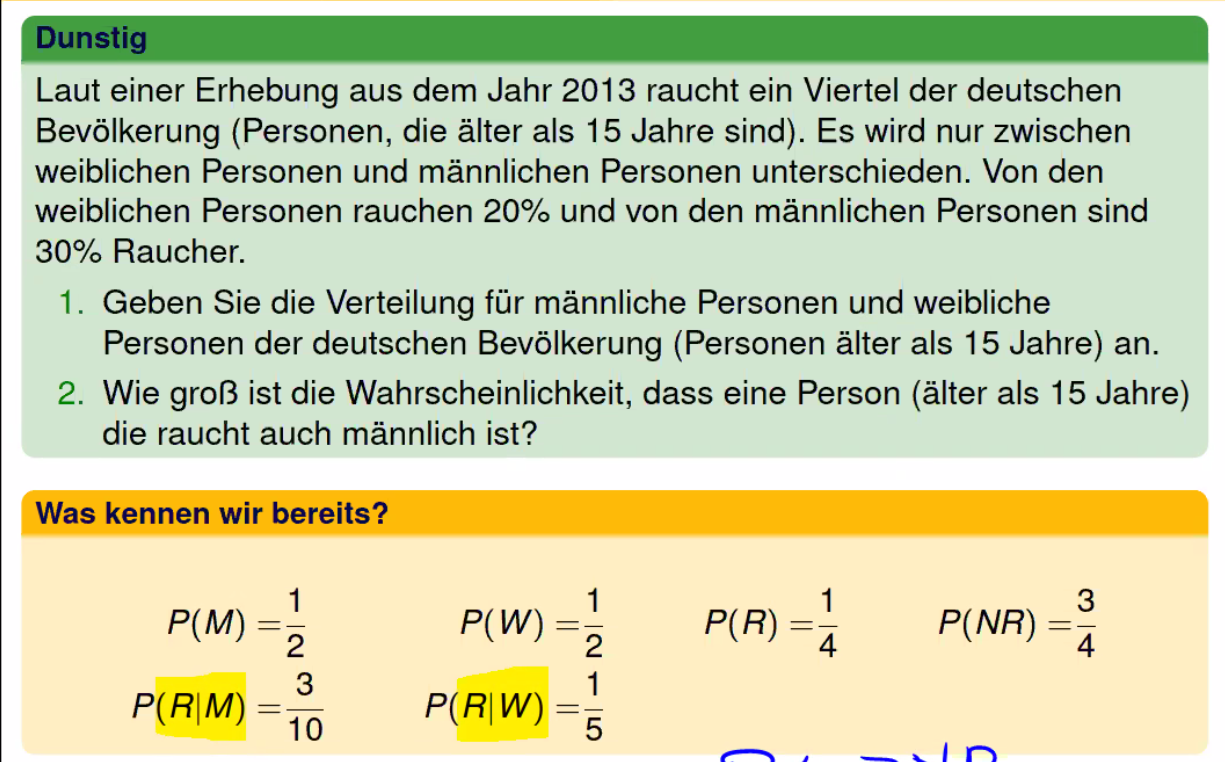
\includegraphics[scale=0.25]{Raucher Stat.png}\\
	Gemeinsame Wahrscheinlichkeit: $P(M\cap NR) = P(NR|M)P(M)$\\
	$P(W\cap NR) = P(NR|W)P(W)$\\
	Wir wissen, dass es nur raucher und nichtraucher gibt, also $P(NR|M) = 1-P(R|M)$, $P(NR|W) = 1-P(R|W)$\\
	$P(M|R) = \frac{P(M\cap R)}{P(R)} =\frac{P(R|M)P(M)}{P(R)}$\\
	$P(W|R) = \frac{P(W\cap R)}{P(R)} = 1-P(M|R)$\\
	\textbf{Also induziert eine Bedingte Wahrscheinlichkeit eine neues Wahrscheinlichkeitsmaß!}\\
	Sind die Eigenschaften (W,M) und (R,NR) stochastisch unabhängig?\\
	für unabhängigkeit muss $P(M)P(R) \stackequal{?}{} P(M\cap R)$ sein.\\
	$\frac{1}{2}\frac{1}{4}\stackequal{?}{} \frac{3}{20}\implies $ die Beiden sind nicht stochastisch unabhängig!\\
	Wenn bekannt ist, dass $P(A\cap C)\neq P(A)P(C)$ (also A und C abhängig sind), kann man sofort folgen, dass $P(A^C\cap C)$ ist stochastisch unabhängig?\\
	Ja: $P(A^c\cap C)= P(A^C|C)P(C)= (1-P(A|C))P(C) = P(C)-P(A|C)P(C) = P(C)-P(A\cap C)$\\
	stochastische Unabhängigkeit mit mehreren Variablen:\\
	Im binären Fall $A,B: P(A\cap B)=P(A)P(B)$\\
	im trinären Fall $A,B,C$ Powerset durchtesten $P(A\cap B), P(A\cap C), P(B\cap C), P(A\cap B\cap C)$\\
	$A=\{(z,k),(z,z)\}, P(A)=\frac{1}{2}$\\
	$B=\{(k,z),(z,z)\}, P(B)=\frac{1}{2}$\\
	$C=\{(k,z),(z,k)\}, P(C)=\frac{1}{2}$\\
	Also sind $P(A\cap B)=\frac{1}{4}$, $P(A\cap C)=\frac{1}{4}$,$P(C\cap B)=\frac{1}{4}$\\
	\textbf{ABER} $P(A\cap B\cap C) = P(\emptyset) =0\neq P(A)P(B)P(C) = \frac{1}{8}$!\\
	Also sind die drei Ereignisse nicht stochastisch unabhängig, sondern nur paarweise stochastisch unabhängig.\\

\end{document}